In the real world images are sometimes affected by noise in a way that makes working with them (or looking at them) difficult. The purpose of this project is therefore look at image restoration on a set of images that are affected by different kinds of defects. The overall task is to minimize the impact of the noise and thereby to improve the quality of the image.\\[0.2cm]
To come up with an analysis and a way to remove (or weaken) the defect, the following considerations are done for each image: 
\begin{itemize}\itemsep-3pt
\item Investigate the image and identify the defect, for example by using the histogram and/or the frequency spectrum of the image.
\item Design a solution that removes or weakens the impact of the defect and investigate the properties of the solution. 
\item Investigate different solution possibilities.
\item Implement and apply the solution(s)
\end{itemize}

At the end the image restored has to be resemble the original image as best as possible. 

\begin{figure}[H]
\centering
        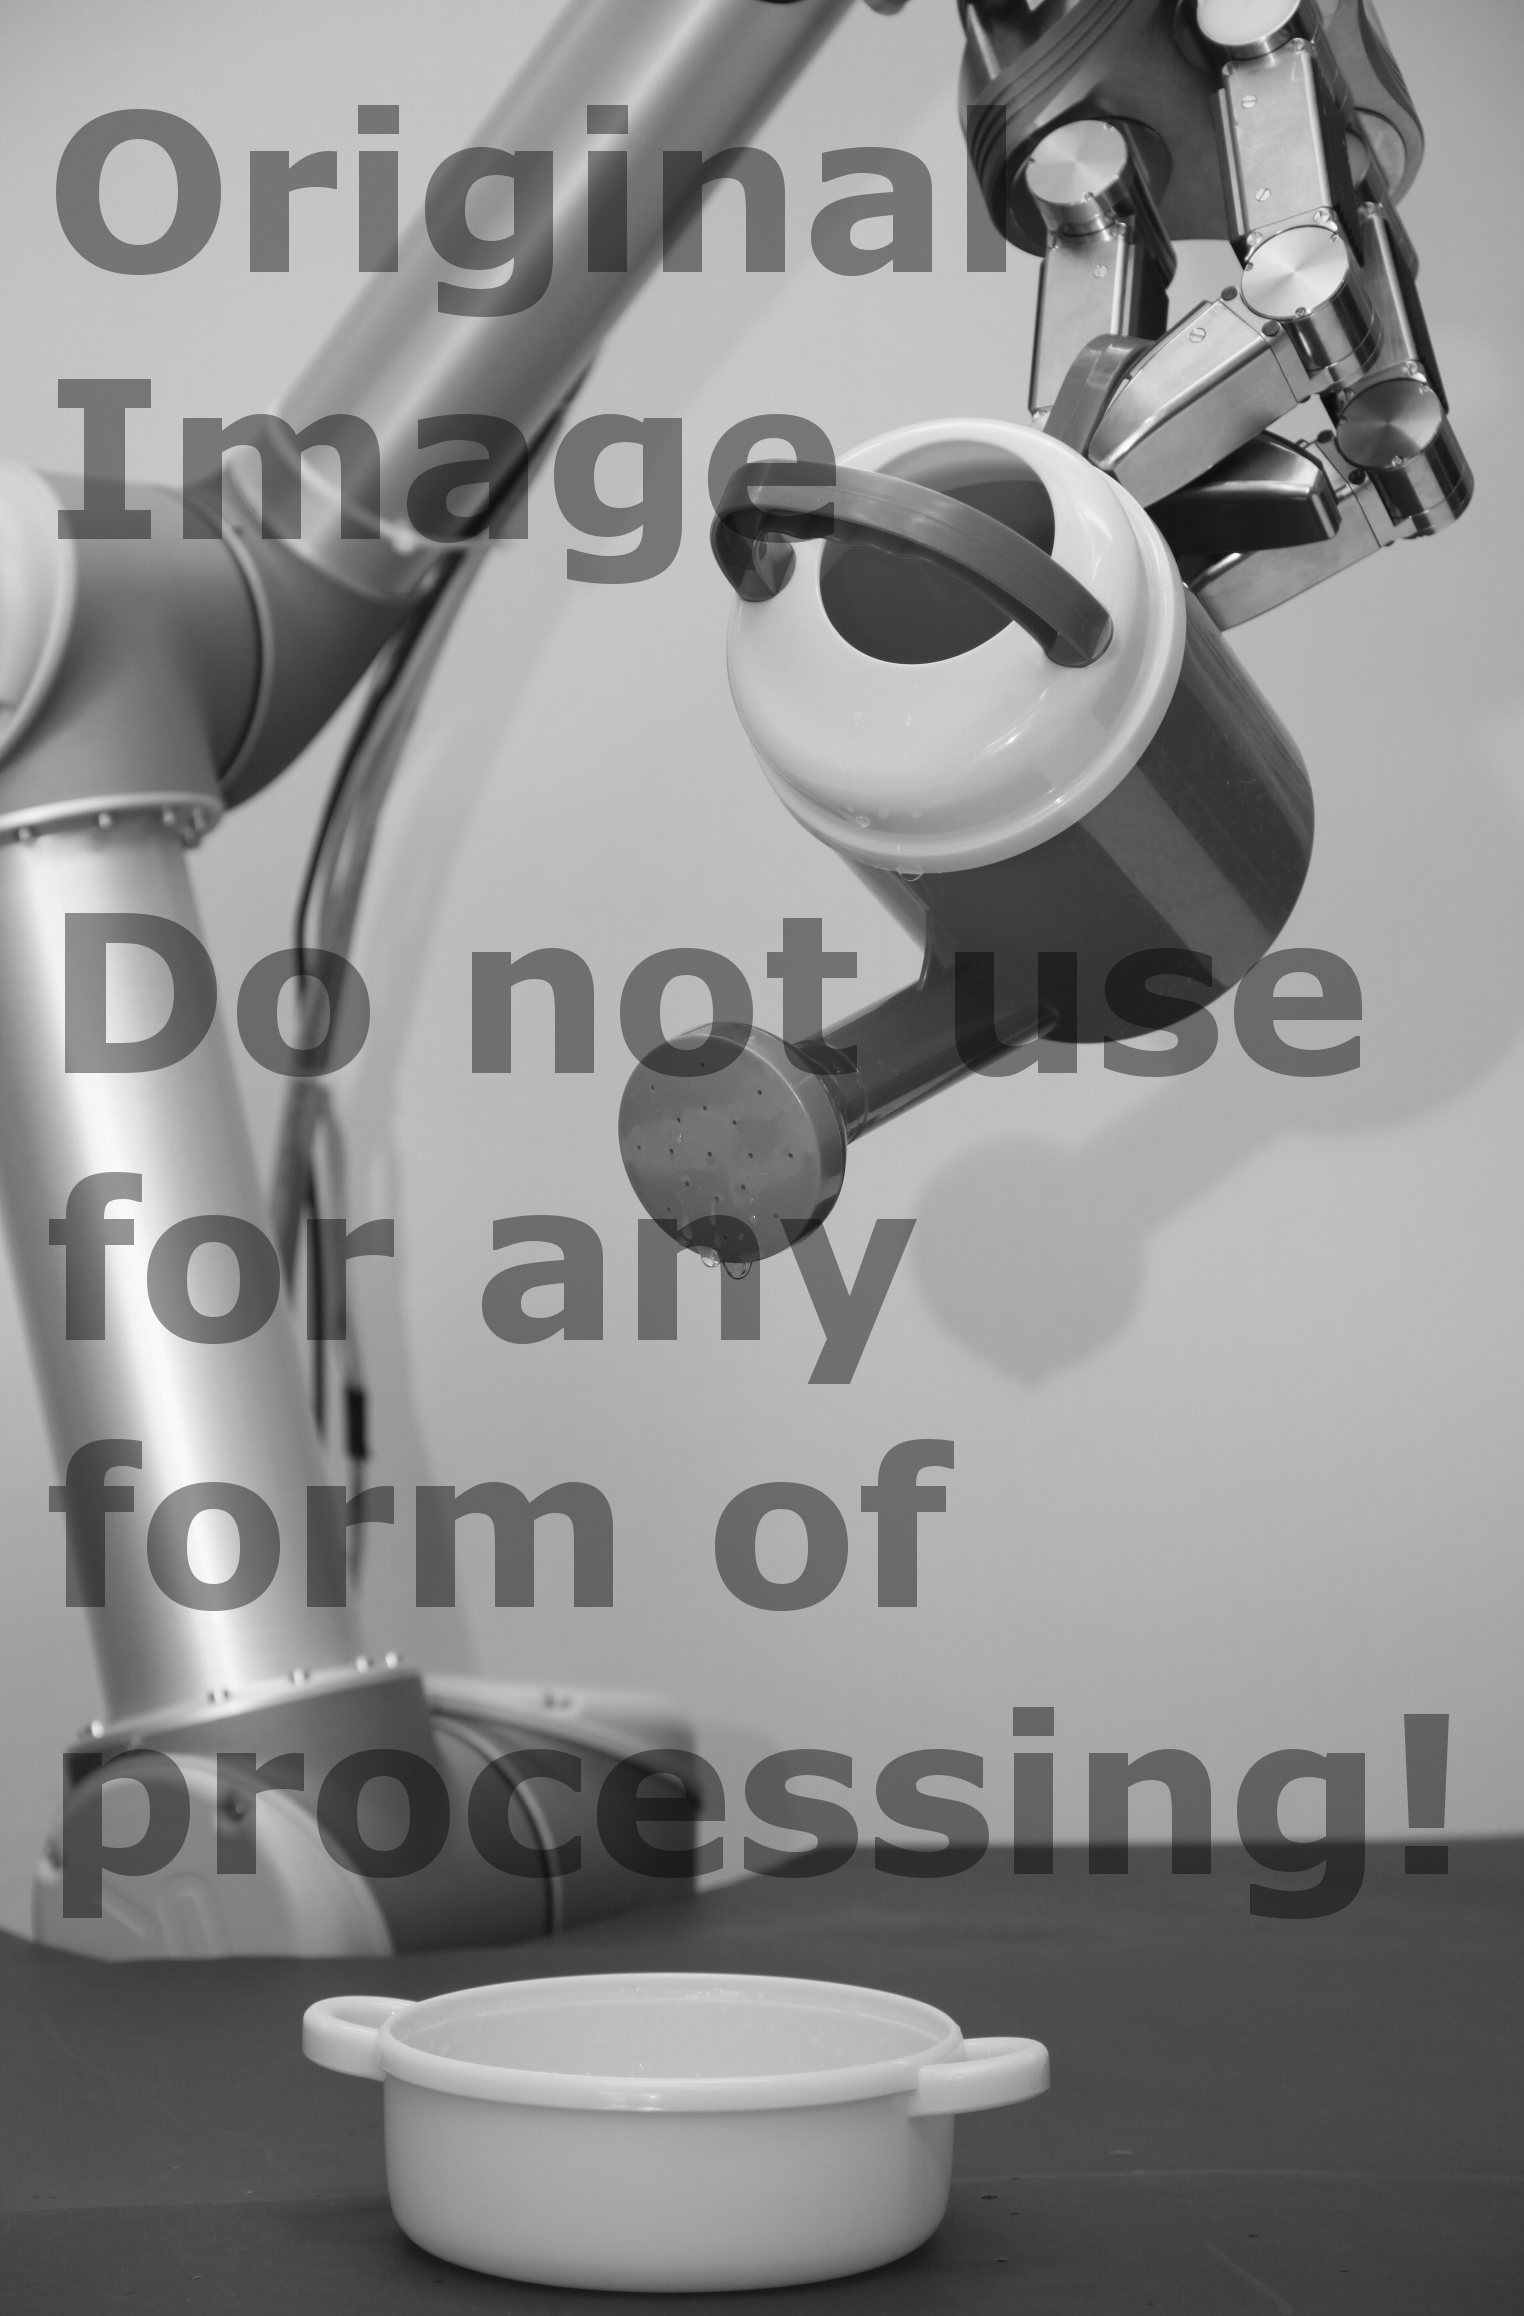
\includegraphics[scale= 0.15]{org.png}
        \caption{The original image}
        \label{fig:orignal}
\end{figure}

